The term $v\cdot \nabla_x f$ makes the distribution $f(v)$ at fixed $(t,x)$ coupled with $f(v)$ defined in neighboring $x$. In operator splitting methods, Boltzmann equation is split in to ``transport'' and ``collision'' part. First we are going to focus on the collision part, given by, 
\begin{equation}
    \partial_t f = \frac{1}{\epsilon}C(f,f) \label{eq:col_op}
\end{equation}
% Note that without the transport term, for fixed $(t,v)$, for $x\neq x_*$ $f(x)$ and $f(x_*)$ can be evolved independently decoupled way. \emph{This allows, spatially subdivision based parallelization algorithms for the Boltzmann equation.}

% \subsection{Properties of the collision operator}
% \label{subsec:collision_op_properties}
% For a given $\R^d$ velocity space,
% \begin{theorem}
%     The Boltzmann collision operator conserves few of it moments, namely, mass, momentum, and energy.
%     \begin{align}
%         \int_{\R^d} Q(f,f) dv  = 0 \\
%         \int_{\R^d} Q(f,f) v dv  = 0 \\
%         \int_{\R^d} Q(f,f) |v|^2dv  = 0 \\
%     \end{align}
% \end{theorem}

% The solution for (\ref{eq:col_op}) evolves towards steady state, defined as the Maxwellian, which is given by, 
% \begin{equation}
%     f_{\infty}(v) = \frac{\rho}{(2\pi T)^{d/2}} \exp{-\frac{|V-v|^2}{2T}}
% \end{equation} where, the Maxwellian depends on the quantities computed from the initial distribution. 

% \begin{itemize}
%     \item \textbf{Density} : $\rho = \int_{\R^d} f(v) dv$ 
%     \item \textbf{Mean/Bulk velocity}: $V=\frac{1}{\rho} \int_{\R^d} v f(v) dv$ 
%     \item \textbf{Temperature}: $T= \frac{1}{3\rho} \int_{\R^d} |V-v|^2 f(v) dv$
% \end{itemize}

\section{Collision operator for electron-neutral elastic collisions}
\label{sec:electron_neutral_pc}
\textcolor{red}{\textbf{Note}}: The below derivation only valid for 2-body elastic collisions. For inelastic collisions require jacobian term in the strong form. Without the proper jacobian term, we the derived weak form does not obey the mass conservation. 
Let $f_e(v,t)$ be the electron density and $f_o(v,t)=\delta(v)$ for all $(t,x)$. Then the evolution of the $f_e$ can be written as, 
\begin{equation}
    \partial_t f_e(v,t) = C(f_e,f_0)
\end{equation}
Let $(v^\prime,v_*^\prime) \rightarrow (v,v_*)$ be the pre and post collision velocities. The assumption $f_o(v,t)=\delta(v)$, implies neutral particles are mostly centered at velocity $0$. We can write the pre collision velocities as, $v^\prime=v^\prime(v,\omega)$. 

With these assumptions, the generic collision operator, for fixed time $t$ can be simplified for follows. 
\begin{align}
    C(f_e,f_0) &= \int_{\R^3}\int_{S^2} B(|v-v_*|,\omega)(f_e(v^\prime)f_0(v_*^\prime) - f_e(v)f_0(v_*) ) d\omega dv_*
\end{align}
Change of the integral order (assumes that the integral is finite) with properties of the Dirac's delta function, we can write, 
\begin{align}
    C(f_e,f_0) &= \int_{S^2} B(|v|,\omega)(f_e(v^\prime) - f_e(v)) d\omega
\end{align}

Then we can write the final evolution equation as, 
\begin{equation}
    \partial_t f_e(v,t) = \int_{S^2} B(|v|,\omega)(f_e(v^\prime,t) - f_e(v,t)) d\omega
\end{equation}

Since we know the above evolution will reach the Maxwellian at $t\rightarrow \infty$, we approximate $f_e(v,t)$ as follows, where $M(v)$ denotes the Maxwellian, 
\begin{equation}
    f_e(v,t) = M(v)[1 + h(v,t)] \label{eq:maxwelian}
\end{equation}
The idea is that when $t\rightarrow \infty$ the time dependent, $h(v,t)\rightarrow 0$.
Assuming that $\phi(v)$ is our test function with required properties. We can write the variational form for the above as, 
\begin{equation}
    \frac{\partial}{\partial t} \int_{\R^3} f_e(v,t) \phi(v) dv = \int_{\R^3} \int_{S^2} B(|v|,\omega)(f_e(v^\prime,t) - f_e(v,t)) \phi(v) d\omega dv \label{eq:0d_wf}
\end{equation}

Let $P_i(v)$ be orthonormal polynomial basis with the weighted inner product in the velocity space, where $w(v)$ denotes tha weight function. 
\begin{align}
    \int_{V} w(v)P_i(v)P_j(v) dv &= k_i\delta_{ij}
\end{align}

Assuming finite dimensional expansion for fixed time $t$, on $f(v,t)$, we can write, 
\begin{equation}
    f(v,t) \approxeq \bar{f}(v,t) = M(v)\sum_{j=0}^{N_v} f_j(t) P_j(v) \label{eq:basis_expansion}
\end{equation}

% Substituting (\ref{eq:basis_expansion}) to (\ref{eq:0d_wf}) we can write, 
% \begin{align}
%     \partial_t \int_{\R^3} w(v)h(v,t)\phi(v) dv &=  \int_{\R^3} \int_{S^2} (M(v^\prime) - M(v)) \phi(v) B(|v|,\omega) d\omega dv\\
%     &+\int_{\R^3} \int_{S^2} (M(v^\prime)h(v^\prime,t) - M(v)h(v,t)) B(|v|,\omega) \phi(v) d\omega dv
% \end{align}
For the above, By substituting, basis expansion for $f(v,t)$ we can write, 
\begin{align}
    \partial_t \int_{\R^3} M(v)\sum_{j=0}^{N_v} f_j(t) P_j(v) \phi(v) dv &= \\\int_{\R^3} \int_{S^2} M(v^\prime)\sum_{j=0}^{N_v} f_j(t) P_j(v^\prime) & B(|v|,\omega) \phi(v) d\omega dv \nonumber \\
    -\int_{\R^3} \int_{S^2} M(v)\sum_{j=0}^{N_v} f_j(t) P_j(v) &B(|v|,\omega) \phi(v) d\omega dv
\end{align}
By choosing $\phi(v) = P_i(v)$, we can further simplify, 
\begin{align}
    \text{diag}(k_i^\prime)\partial_t{f_i} = \sum_{j=0}^{N_v} L_{ij} f_j(t)
\end{align} where, 
\begin{equation}
    L_{ij} = \int_{\R^3} \int_{S^2} (M(v^\prime) P_i(v)P_j(v^\prime)  - M(v) P_i(v) P_j(v) )  B(|v|,\omega) d\omega dv
\end{equation}
\begin{equation}
    k_{i}^\prime = \int_{\R^3} M(v) P_i(v)^2 dv
\end{equation}

\subsection{Issue of mass conservation when used in inelastic collisions}
For any smooth distribution, $f(v) = M(v_\alpha) \sum_{klm} f_{klm} \phi_{klm}(v_\alpha)$, and we can write, 
\begin{align}
\int_{\RR^3} f dv &= const.  \\
\frac{d}{dt} \int_{\RR^3} f dv &= 0  \\
\int_{\RR^3} \partial_t f  dv &= \int_{\RR^3} c(f) dv =0 \\
% \partial_t f &= c(f) = n_0 \int_{S^2} (f(v^\prime) - f(v)) \norm{v} \sigma(\norm{v},\omega) d\omega \\
% \frac{d}{dt} \int_{\RR^3} f dv =0  &\implies \int_{\RR^3} c(f) dv = 0 
\end{align}
We can further write, 
\begin{align}
\int_{\RR^3} c(f) dv  &= \sum_{klm} f_{klm} \int_{\RR^3}\int_{S^2} \bigl( M(v^\prime/\alpha) \phi_{klm}(v^\prime/\alpha) -   M(v/\alpha) \phi_{klm}(v/\alpha) \bigr) \\ &\times\norm{v} \sigma(\norm{v},\omega) d\omega dv, \  \forall f(v,t) \\
\implies & \int_{\RR^3}\int_{S^2} \bigl( M(v^\prime/\alpha) \phi_{klm}(v^\prime/\alpha) -   M(v/\alpha) \phi_{klm}(v/\alpha) \bigr) \norm{v} \\ \times &\sigma(\norm{v},\omega) d\omega dv =0  \forall klm
\end{align}
But the above is not satisfied, take const polynomial $\phi_{000}(x)=1/2\sqrt{\pi}$ with $v^\prime \neq v$.
%For radial advection we can write, 
%\begin{align*}
%&\myint_{V} v^2 \partial_v f_{lm} \psi_p(t) dv = \myint_{V} v^2 \partial_v \sum_{k} f_{klm} \exp(-x^2) \phi_k(t) \psi_p(t) dv =W_{pk} f_{lm} \\
%W_{pk} &= \myint_{V} v^2 \partial_v \of{\exp\of{-x^2} \phi_k\of{t}}\psi_p\of{t} dv\\
%\myint_{V} v^2 \partial_v f_{lm} \psi_p(t) dv &=\myint_{\partial V} v^2 f_{lm}^* \of{v} \psi_p\of{t} ds - \myint_{V} f_{lm}\of{v} \of{v^2 \partial_v\psi_p\of{t} + \psi_p\of{t} 2v } dv \\
%&D^{p}_{k}= \myint_{V} v^2 \exp(-x^2) \phi_{k}\of{t} \partial_v \psi_p\of{t} dv \\
%&D^{p}_{k}= v_{th}^2\myint_{V} x^2 \exp(-x^2) \phi_{k}\of{t} \partial_x \psi_p\of{t} dx \\
%&S^{p}_{k}= \myint_{V} v \exp(-x^2) \phi_{k}\of{t}\psi_p\of{t} dv = v_{th}^2 \myint_{V} x \exp(-x^2) \phi_{k}\of{t}\psi_p\of{t} dx \\
%\myint_{V} v^2 \partial_v f_{lm} \psi_p(t) dv &=\myint_{\partial V} v^2 f_{lm}^* \of{v} \psi_p\of{t} ds -(D^{p}_{k} + 2S^{p}_{k}) f_{klm}
%\end{align*}
%
%\begin{align*}
%M^{pqs}_{klm}\partial_t f_{klm} -E A^{qs}_{lm} \of{\myint_{\partial V} v^2 f_{lm}^* \of{v} \psi_p\of{t} ds}  + E A^{qs}_{lm}(D^{p}_{k} + 2S^{p}_{k})f_{klm} -E B^{qs}_{lm} S^{p}_{k}f_{klm}  = C^{pqs}_{klm}f_{klm}
%\end{align*}

%\subsection{Bolsig collision approximation}
%For gas temperature $T=0$ we can write the collision operator as, 
%\begin{align*}
%C_{G0} &= \gamma \frac{2m}{M} \partial_{\varepsilon} \of{\varepsilon^2 \sigma f \of{\varepsilon}} \text{ and } \varepsilon = \of{\frac{v}{\gamma}}^2 \\
%f\of{\varepsilon,\omega}&= \sum_{klm} f_{klm} \phi_{klm}\of{\frac{\sqrt{\varepsilon}\gamma}{v_{th}},\omega} \\
%\myint_{\R^3} C_{G0} \psi_{pqs}\of{\vect{v}} \diff{\vect{v}} & = \myint_{R^3}  \gamma \frac{2m}{M} \partial_{\varepsilon} \of{\varepsilon^2 \sigma f \of{\varepsilon}} \psi_{pqs}\of{\frac{\vect{v}}{v_{th}}} \diff{\vect{v}}\\
%{C_{G0}}_{klm}^{pqs} &= \gamma \frac{2m}{M}  \myint_{\R^3} \partial_{\varepsilon}\of{\varepsilon^2 \sigma \phi_{klm}\of{\frac{\sqrt{\varepsilon}\gamma}{v_{th}},\omega}} \psi_{pqs}\of{\frac{\vect{v}}{v_{th}}} \diff{\vect{v}}
%\end{align*} 
%\begin{align*}
%&{C_{G0}}_{klm}^{pqs} = \gamma \frac{2m}{M} \myint_{\R^+} 
%v^2  \partial_{\varepsilon}\of{\varepsilon^2 \sigma \phi_{k}\of{\frac{v}{v_{th}}}}  \psi_{p}\of{\frac{v}{v_{th}}} \diff{v} \delta^{q}_{l} \delta^{s}_{m}\\
%&{C_{G0}}_{klm}^{pqs} = \gamma \frac{2m}{M} 
%\myint_{\R^+} 
%v^2  \of{
%	\varepsilon^2 \sigma \partial_{\varepsilon} \phi_{k}\of{\frac{v}{v_{th}}} +
%	 \of{
%		2\varepsilon \sigma + \varepsilon^2 \partial_{\varepsilon} \sigma 
%	 }
%	 \phi_{k}\of{\frac{v}{v_{th}}}
%}\psi_{p}\of{\frac{v}{v_{th}}} \diff{v} \delta^{q}_{l} \delta^{s}_{m} \\
%&x=\frac{v}{v_{th}} \text{ , }  \varepsilon = \of{\frac{x v_{th}}{\gamma}}^2  = \of{\frac{v}{\gamma}}^2 \implies \frac{dx}{d\varepsilon} = \frac{x}{2\varepsilon}\\
%&{C_{G0}}_{klm}^{pqs} = \frac{2m v_{th}^5 } {M\gamma} \of{
%	\myint_{\R^+} \frac{1}{2} x^5 \sigma \partial_x \phi_k\of{x} \psi_p\of{x} dx +
%	\myint_{\R^+} x^4 \of{2\sigma + \varepsilon \partial_{\varepsilon}\sigma} \phi_{k}\of{x} \psi_p\of{x} dx 	
%} \delta^{q}_{l} \delta^{s}_{m}
%\end{align*}




\newpage
%diagonalization (manually try to diagonalize, hard to keep track of the other terms. )?
%\begin{align*}
%\frac{d}{dt} \left( f_{0,0} + f_{1,0} \right) - E 
%\left( \frac{1}{\sqrt{3}} \frac{d}{d\vr} \left( f_{0,0} + f_{1,0} \right) 
%+  \frac{2}{\sqrt{3}} \frac{1}{\vr} f_{1,0} \right) &= \ldots
%\\
%\frac{d}{dt} \left( f_{0,0} - f_{1,0} \right) - E 
%\left( - \frac{1}{\sqrt{3}} \frac{d}{d\vr} \left( f_{0,0} - f_{1,0} \right) 
%+  \frac{2}{\sqrt{3}} \frac{1}{\vr} f_{1,0} \right) &= \ldots
%\end{align*}
%
%Let $F_0\of{v} = f_{0,0}\of{v} + f_{1,0}\of{v}$ and $F_1\of{v} = f_{0,0}\of{v} - f_{1,0}\of{v}$ and $c=\frac{E}{\sqrt{3}}$. 
%\begin{align*}
%\partial_t F_0  - c \partial_v F_0 + 2c \frac{1}{v} f_{1,0} &= ... \\
%\partial_t F_1  + c \partial_v F_1 + 2c \frac{1}{v} f_{1,0} &= ...
%\end{align*} Projects to $\psi\of{v}$ radial test functions for $v\in V =[v_L,v_R]\subset [0,\infty]$.
%\begin{align*}
%\myint_{V} \partial_t F_0 \of{v} v^2 \psi\of{v} \diff{v} -& c \myint_{V} \partial_v F_0 \of{v} v^2 \psi\of{v}\diff{v} + 2c \myint_{V} v f_{1,0} \of{v} \psi\of{v} dv = ... \\
%\myint_{V} \partial_t F_0 \of{v} v^2 \psi\of{v} \diff{v}  -c  &\Big[F_0\of{v} v^2 \psi\of{v}\Big]_{v_L}^{v_R}  + c \myint_{V} F_0\of{v} \left(v^2\partial_v \psi\of{v} + 2v\psi\of{v}\right) dv\\
% +& 2c \myint_{V} v f_{1,0} \of{v} \psi\of{v} dv = ... \\
%\end{align*}
%Similarly for $F_1\of{v}$ we can write, 
%\begin{align*}
%\myint_{V} \partial_t F_1 \of{v} v^2 \psi\of{v} \diff{v}  +c  \Big[F_1\of{v} v^2 \psi\of{v}\Big]_{v_L}^{v_R}  - c \myint_{V} F_1\of{v} \left(v^2\partial_v \psi\of{v} + 2v\psi\of{v}\right) dv\\ + 2c \myint_{V} v f_{1,0} \of{v} \psi\of{v} dv = ...
%\end{align*}
%
%For the domain $D=[D_l,D_r]$ let $\phi_{k}\of{\frac{v}{v_{th}}}$ be the trial functions for expansion and $\psi_{p}\of{\frac{v}{v_{th}}}$ be the corresponding test functions. Let $F_0\of{v}=\sum_{k} h_k \phi_k\of{\frac{v}{v_{th}}}$ and  $F_1\of{v}=\sum_{k} g_k \phi_{k}\of{\frac{v}{v_{th}}}$. Notice that $f_{0,0} = \frac{1}{2}(F_{0} + F{1})$, $f_{1,0} = \frac{1}{2}(F_{0} - F{1})$.
%Using the above expansion and discretizing the above we can write, 
%\begin{align*}
%M_{pk} \partial_t \vect{h}  - c v_{th}^2 \Big[\vect{h}^* \of{\frac{v}{v_{th}}}^2 \boldsymbol{\psi}\of{\frac{v}{v_{th}}}\Big]_{D^l}^{D^{r}} + c (D_{pk} + 2 S_{pk}) \vect{h} + c S_{pk} (\vect{h}-\vect{g})  &= ... \\
%M_{pk} \partial_t \vect{g}  + cv_{th}^2 \Big[\vect{g}^* \of{\frac{v}{v_{th}}}^2 \boldsymbol{\psi}\of{\frac{v}{v_{th}}}\Big]_{D^l}^{D^{r}} - c (D_{pk} + 2 S_{pk}) \vect{g} + c S_{pk} (\vect{h}-\vect{g})  &= ... \\
%\end{align*} where the corresponding operators are defined as bellow (with $x=\frac{v}{v_{th}}$ normalized coordinates). 
%\begin{align*}
%	M_{pk} &= v_{th}^3\myint_{D} x^2 \psi_{p}\of{x} \phi_{k}\of{x} dx \\
%	D_{pk} &= v_{th}^2\myint_{D} x^2 \partial_v \psi_{p}\of{x} \phi_{k}\of{x} dx \\
%	S_{pk} &= v_{th}^2\myint_{D} x \psi_{p}\of{x} \phi_{k}\of{x} dx \\
%	\boldsymbol{\psi}(x)&=[\psi_0(x), ... , \psi_{N}(x)]^T
%\end{align*} The source terms (RHS) of the equations should come from the collision operator. The collision operator with the above basis function can be written as,
%Assuming $f_0\of{\vect{v_0}}=\delta(\vect{v_0}-\vect{0})$, 
%\begin{align*}
%C^- = \myint_{R^3} \myint_{S^2}  
%B\of{\vect{v}_e^\prime, \vect{0}, \vect{\omega}} 
%f_e\of{\vect{v}_e^\prime} \delta\of{\vect{v}_e^\prime - \vect{v}_e} 
%\diff{\vect{v}_e^\prime} \diff{\vect{\omega}}. \\
%\end{align*} Let $B_0(\cdot,\cdot) \equiv B(\cdot,\vect{0},\cdot)$, then projecting into spherical harmonics, 
%\begin{align*}
%\myint_{S^2} C^- Y(\omega_{v_e}) \diff{\omega_{v_e}}& = 
%\myint_{R} \myint_{S^2} \myint_{S^2} 
%{v_e^\prime}^2 B_0\of{(v_e^\prime,\vect{\omega_{v_e}}), \vect{\omega}} \times \\
%&f_e\of{(v_e^\prime,\vect{\omega_{v_e}})} \delta\of{v_e^\prime - v_e} Y\of{\vect{\omega_{v_e}}} 
%\diff{v_e^\prime} \diff{\vect{\omega_{v_e}}} \diff{\vect{\omega}}. \\
%\end{align*} Similarly we can write the gain term, 
%\begin{align*}
%C^+ = \myint_{R^3} \myint_{S^2}  
%B_0\of{\vect{v}_e^\prime, \vect{\omega}} 
%f_e\of{\vect{v}_e^\prime} \delta\of{\vect{v}_e^{post}(\vect{v_e}^\prime,\vect{0},\omega)- \vect{v}_e} 
%\diff{\vect{v}_e^\prime} \diff{\vect{\omega}} 
%\end{align*}
%\begin{align*}
%\myint_{S^2} C^+ Y(\omega_{v_e}) \diff{\omega_{v_e}}& = \myint_{R} \myint_{S^2} \myint_{S^2}
%B_0\of{(v_e^\prime,\omega_{v_e}^\prime), \vect{\omega}} {v_e^\prime}^2 \times \\
%&f_e\of{(v_e^\prime,\omega_{v_e}^\prime)} \delta\of{v_e^{post}((v_e^\prime,\omega_{v_e}^\prime),\omega)- {v}_e} Y\of{\omega_{v^{post}}} \diff{v_e^\prime} \diff{\vect{\omega_{v_e}^\prime}} \diff{\vect{\omega}}\\
%&=\myint_{R} \myint_{S^2} \myint_{S^2}
%B_0\of{(v_e^\prime,\omega_{v_e}), \vect{\omega}} {v_e^\prime}^2 \times \\
%&f_e\of{(v_e^\prime,\omega_{v_e})} \delta\of{v_e^{post}((v_e^\prime,\omega_{v_e}),\omega)- {v}_e} Y\of{\omega_{v^{post}}} \diff{v_e^\prime} \diff{\vect{\omega_{v_e}}} \diff{\vect{\omega}}
%\end{align*} Therefore, combined collision operator can be written as, 
%\begin{align*}
%\myint_{S^2} C Y\of{\omega_{v_e}} \diff{\omega_{v_e}}& = 
%\myint_{R} \myint_{S^2} \myint_{S^2} 
%B_0\of{(v_e^\prime,\omega_{v_e}), \vect{\omega}} {v_e^\prime}^2 f_e\of{(v_e^\prime,\omega_{v_e})} \times \\
%\Bigg(
%&\delta\of{v_e^{post}- {v}_e} Y\of{\omega_{v^{post}}} - \delta\of{v_e^\prime - v_e} Y\of{\omega_{v_e}}
%\Bigg)
%\diff{\vect{\omega}} \diff{\vect{\omega_{v_e}}} \diff{v_e^\prime} 
%\end{align*} 
%\begin{align*}
%C^{pqs}_{klm} &= \myint_{V}\myint_{S^2}\myint_{S^2} B_0\of{(v_e,\omega_{v_e}), \vect{\omega}} {v_e}^2 \\
%&\phi_{k}\of{v} Y_{lm}(\omega_{v_e}) \Bigg( \psi_p\of{v^{post}_e} Y_{qs}\of{\omega_{v^{post}}} -\psi_{p}(v_e)Y_{qs}\of{\omega_v} \Bigg) \diff{v_e} \diff{\omega_{v_e}}\diff{\omega}
%\end{align*}.
%We can write, 
%\begin{align*}
%M_{pk} \partial_t \vect{h}  - c v_{th}^2 \Big[\vect{h}^* \of{\frac{v}{v_{th}}}^2 \boldsymbol{\psi}\of{\frac{v}{v_{th}}}\Big]_{D^l}^{D^{r}} + c (D_{pk} + 2 S_{pk}) \vect{h} + c S_{pk} (\vect{h}-\vect{g})  &= C^{p00}_{k00} \frac{1}{2} (\vect{h} + \vect{g}) + C^{p00}_{k10} \frac{1}{2} (\vect{h} - \vect{g})  \\
%M_{pk} \partial_t \vect{g}  + cv_{th}^2 \Big[\vect{g}^* \of{\frac{v}{v_{th}}}^2 \boldsymbol{\psi}\of{\frac{v}{v_{th}}}\Big]_{D^l}^{D^{r}} - c (D_{pk} + 2 S_{pk}) \vect{g} + c S_{pk} (\vect{h}-\vect{g})  &= C^{p10}_{k00} \frac{1}{2} (\vect{h} + \vect{g}) + C^{p10}_{k10} \frac{1}{2} (\vect{h} - \vect{g}) \\
%\end{align*} %where $F^*_{\{0,1\}}$ denotes the flux terms for domain boundaries. 
%
%\begin{align*}
%\begin{bmatrix}
%M_{pk} & 0      \\
%0      & M_{pk} 
%\end{bmatrix} \partial_t \vect{F} &= -\begin{bmatrix}
%c(D_{pk} + 3S_{pk}) & -cS_{pk} \\
%cS_{pk} & -c(D_{pk} + 3S_{pk})
%\end{bmatrix} \vect{F}   + \begin{bmatrix}
%\frac{C^{p00}_{k00} + C^{p00}_{k10} }{2} & \frac{C^{p00}_{k00} - C^{p00}_{k10} }{2} \\
%\frac{C^{p10}_{k00} + C^{p10}_{k10} }{2} & \frac{C^{p10}_{k00} - C^{p10}_{k10} }{2} \\
%\end{bmatrix}\vect{F} - W\vect{F^*}
%\end{align*} where $\vect{F}=[\vect{h},\vect{g}]^T$, with $F^*$ denotes the flux terms, coupling the discontinuous domains.  






\newpage
\section{Numerical evaluation}
This section presents, a numerical evaluation of the spatially homogeneous Boltzmann equation without external force field. Recall, under the above assumptions we can write the collision source term as \eqref{eq:nr_be}, 
\begin{equation}
\partial_t f_e(v,t) = \sum_{k} n_k C_k(f_e) \label{eq:nr_be}
\end{equation} where the $C_k$ denotes the collision operator for the $k^{th}$ collision. We consider the following experiments in the study. 
\begin{itemize}
	\item G0: $e + Ar \rightarrow e + Ar $ 
	\item G1: $e + Ar \rightarrow e + Ar^*$
	\item G2: $e + Ar \rightarrow e + Ar^+ + e$ 
\end{itemize} The post collision velocities for the above collisions are summerized in \S\ref{sec:col_op_torch}.


\subsection{Handling changing temperature}
Due to the kinetic energy loss in $e-Ar$ collisions, the thermal velocity decreases with the time. Since we use quadrature points on the normalized velocity (i.e., $\frac{v}{v_th}$) we need transform the solution from one temperature to another. If the temperature drop is significant and if we don't have enough basis functions in the radial direction, the projection between temperature cause an aliasing effect and gives larger tails. 

Let $T_\alpha$ be the current temperature and we want to transform the solution to $T_\beta=T_\alpha (1+ \epsilon)$ where $\epsilon \in [-a,a]$ for $a>0$.

\begin{align}
W_{ij} &= \int_{\reals} M(v_\alpha) P_i(v_\beta) P_j(v_\alpha)dv \label{eq:basis_change}
\end{align}
Let $\epsilon >0$, $\alpha = \beta + \epsilon$. Then we can write the simplified $W_{ij}$ as, 
\begin{align}
W_{ij} &= \frac{n}{\sqrt{\pi}^{3}}  \int_{\reals}  \exp(-v_\alpha^2) P_i (v_\alpha (1 + \frac{\epsilon}{\beta})) P_j(v_\alpha) \frac{dv}{\alpha} \\
\end{align}

\begin{figure}[!htbp]
	\centering
	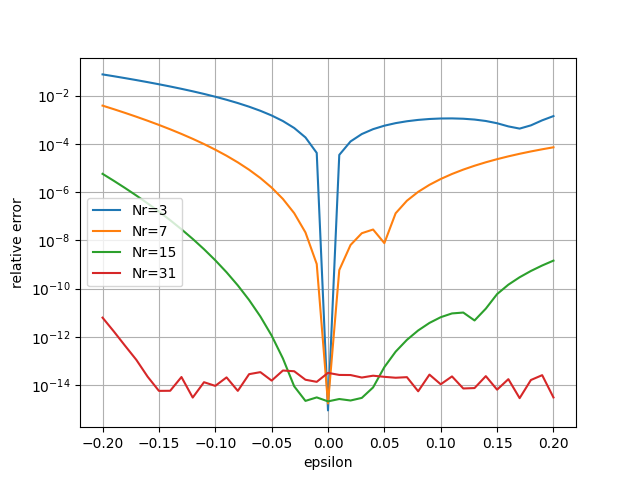
\includegraphics[width=0.48\textwidth]{fig/basis_1ev_grid.png}
	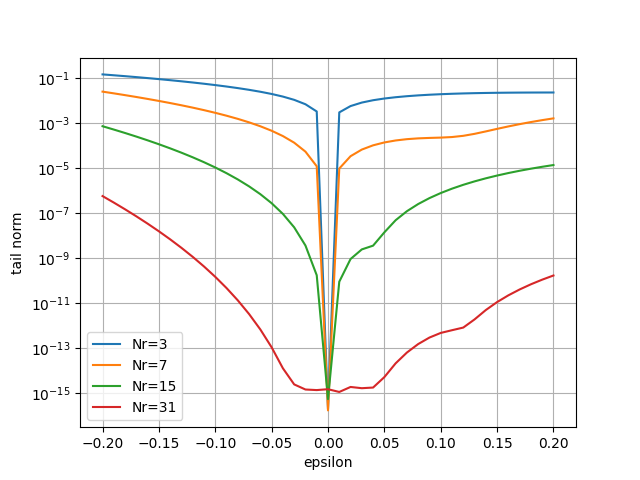
\includegraphics[width=0.48\textwidth]{fig/basis_1ev_tail.png}
	\caption{The left most figure shows the $f(v)$ expansion evaluated at uniform grid in the radial direction followed by normed difference computation for increasing $N_r$ polynomials. For a given Maxwellian distribution (i.e., $h^{\alpha}=1$) we compute the projection of the solution to $T_\beta=T_\alpha (1+\epsilon)$ with computed $W_{\beta\alpha}$, where $h^{\beta} = W_{\beta \alpha} h^{\alpha}$. The right most figure shows the tail of the computed $h^{\beta}$ with increasing polynomials in the radial direction.  \label{fig:basis_projection_error}
	}
\end{figure}
\begin{figure}[!hbtp]
	\centering
	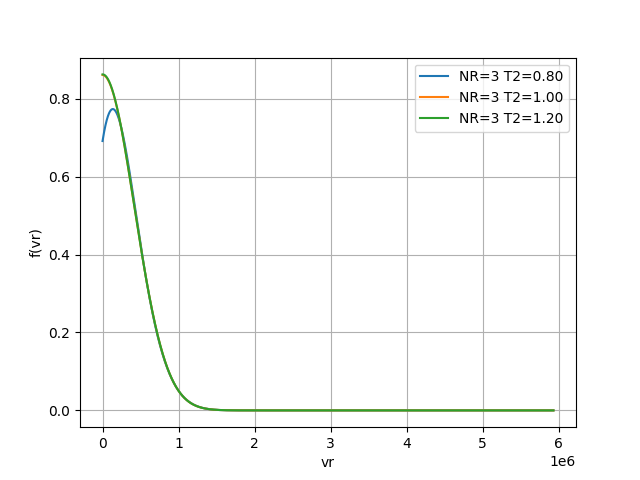
\includegraphics[width=0.48\textwidth]{fig/basis_1ev_f_NR_3.png}
	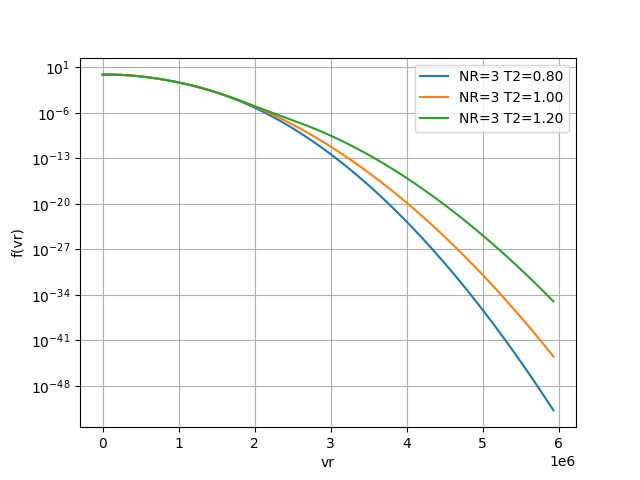
\includegraphics[width=0.48\textwidth]{fig/basis_1ev_log_f_NR_3.png}
	
	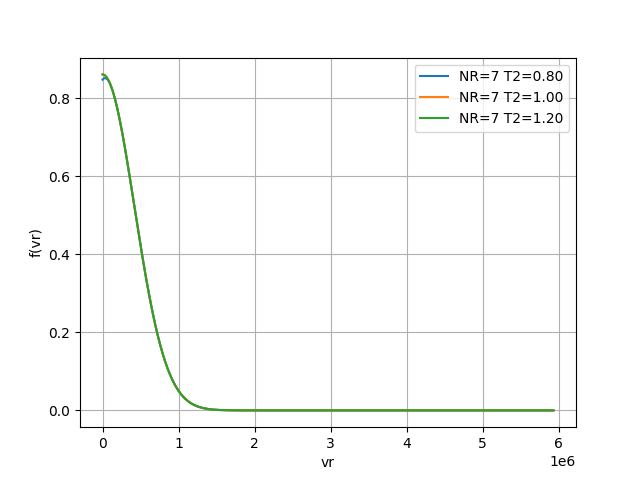
\includegraphics[width=0.48\textwidth]{fig/basis_1ev_f_NR_7.png}
	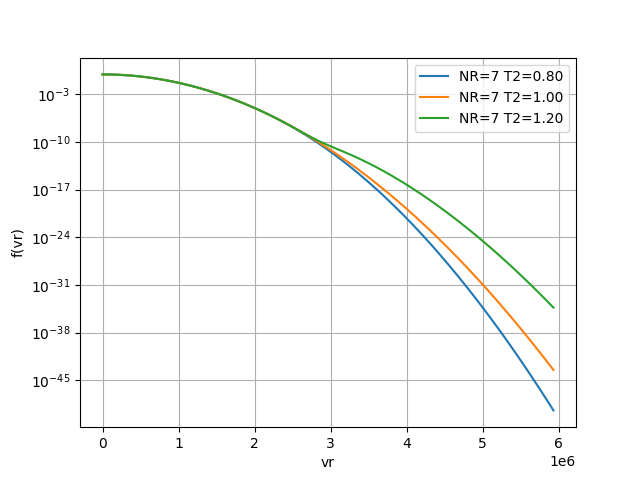
\includegraphics[width=0.48\textwidth]{fig/basis_1ev_log_f_NR_7.png}
	
	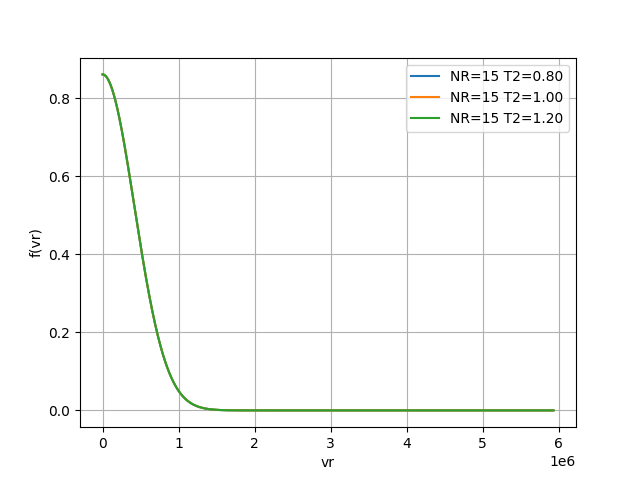
\includegraphics[width=0.48\textwidth]{fig/basis_1ev_f_NR_15.png}
	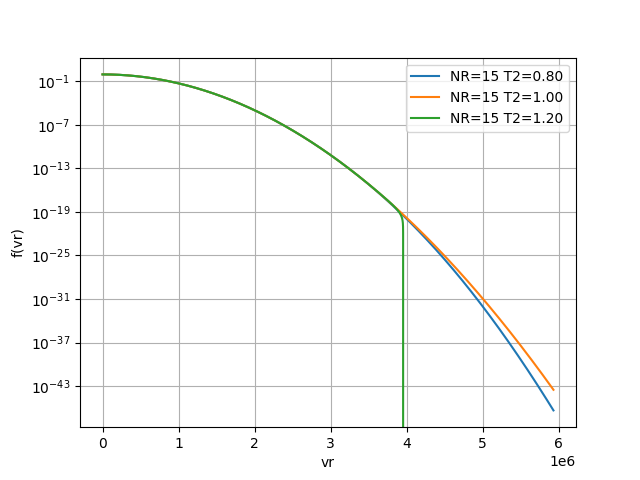
\includegraphics[width=0.48\textwidth]{fig/basis_1ev_log_f_NR_15.png}
	
	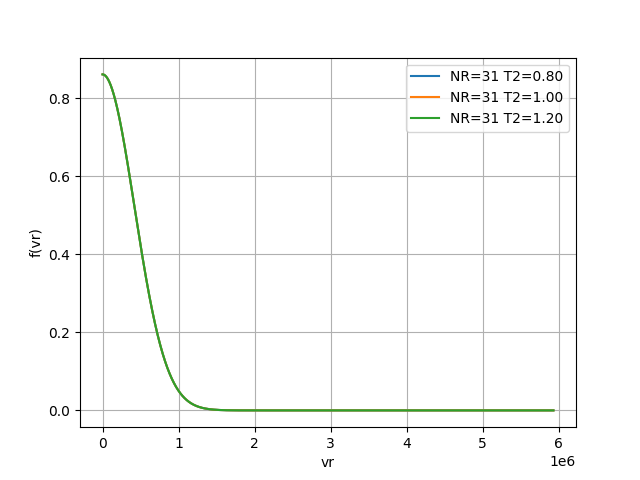
\includegraphics[width=0.48\textwidth]{fig/basis_1ev_f_NR_31.png}
	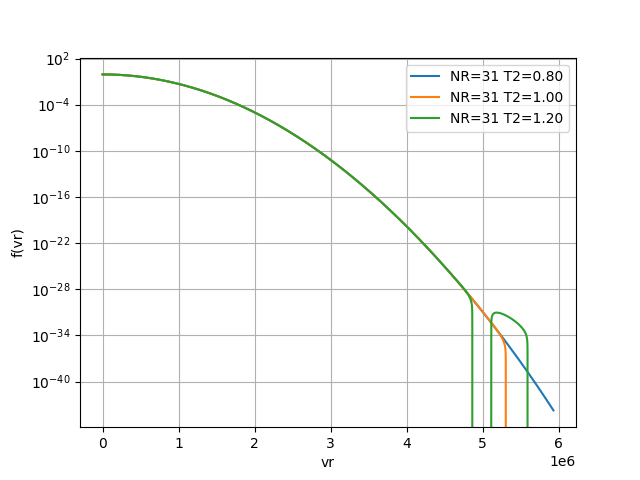
\includegraphics[width=0.48\textwidth]{fig/basis_1ev_log_f_NR_31.png}
	\caption{ For each row the the right most figure shows the log scale to emphasis the variation in the tails of the distribution function. Each row corresponds to a temperature change indicated byt the $\epsilon$ parameter, and projected coefficient evaluated at a uniformly space grid of $10^5$ points in the range of $(0,6V_th)$. 
		\label{fig:basis_grid_plot}
	}
\end{figure}


\newpage
\section{Numerical results with picewise linear synthetic cross section data}
Experimental setup summary. 
\begin{itemize}
	\item Collision operator assembled using composite Simpson rule with 1601 points in the radial direction. 
\end{itemize}
\begin{figure}[!tbhp]
	\centering
	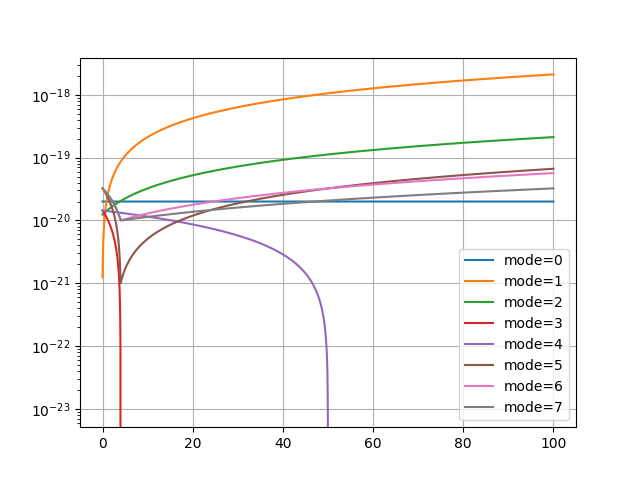
\includegraphics[width=0.8\textwidth]{fig/dat_1ev_cs.png}
	\caption{Total cross-section plots with different synthetic functions. For modes 3,4,5,6 the kink is at an exact quadrature point while mode 7 kink location is not co-located with a quadrature point. For all the experiment differential cross-section computed with uniform distribution.}
\end{figure}
\begin{figure}[!htbp]
	\centering
	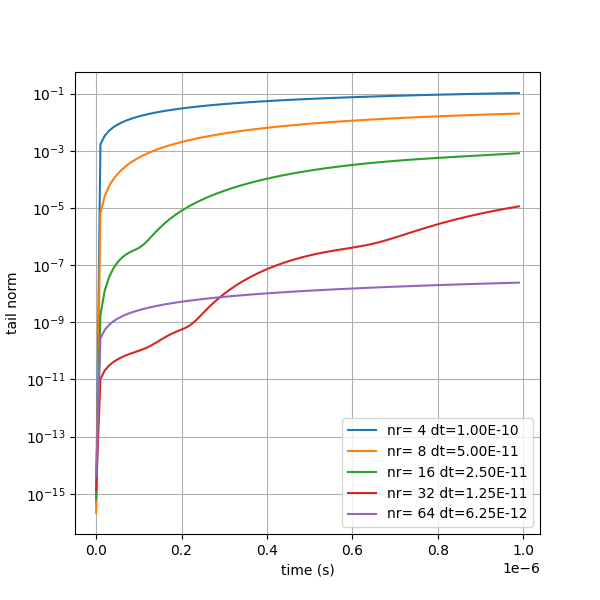
\includegraphics[width=0.32\textwidth]{fig/dat_1ev_cs_m0_tail.png}
	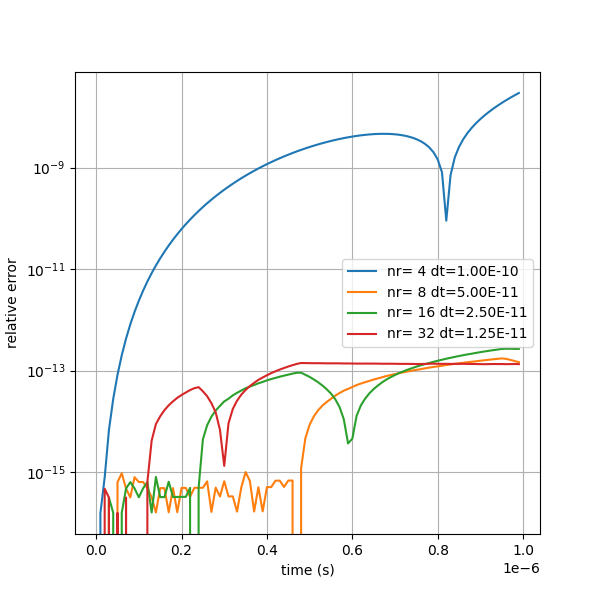
\includegraphics[width=0.32\textwidth]{fig/dat_1ev_cs_m0_temp_error.png}
	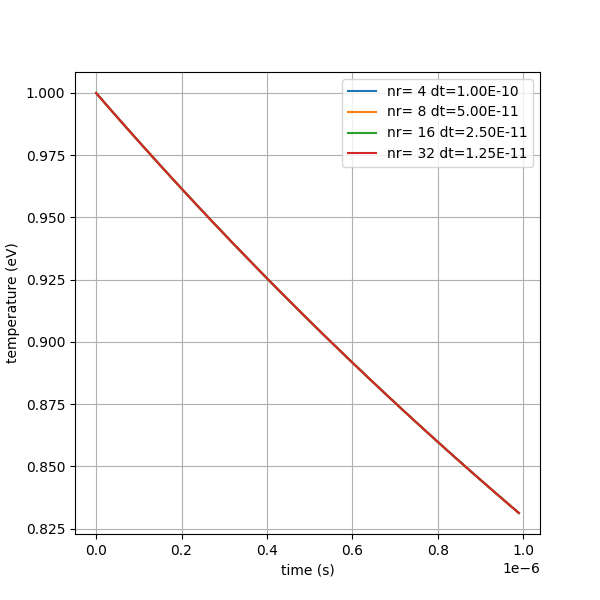
\includegraphics[width=0.32\textwidth]{fig/dat_1ev_cs_m0_temp.png}
	\caption{Mode 0}
\end{figure}
\begin{figure}[!htbp]
	\centering
	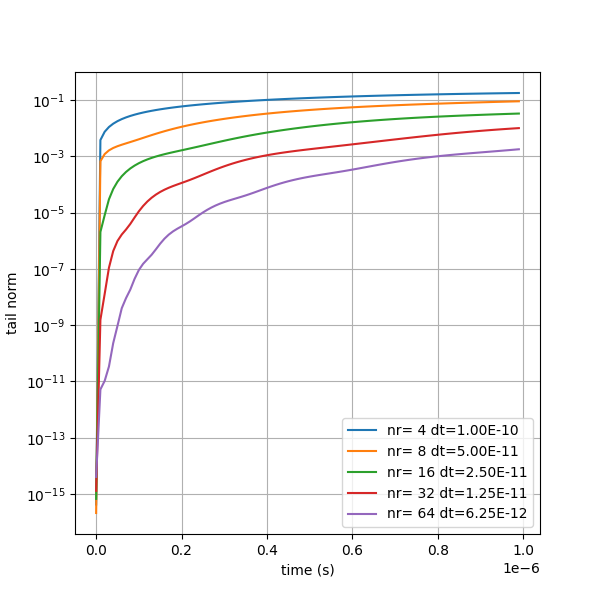
\includegraphics[width=0.32\textwidth]{fig/dat_1ev_cs_m1_tail.png}
	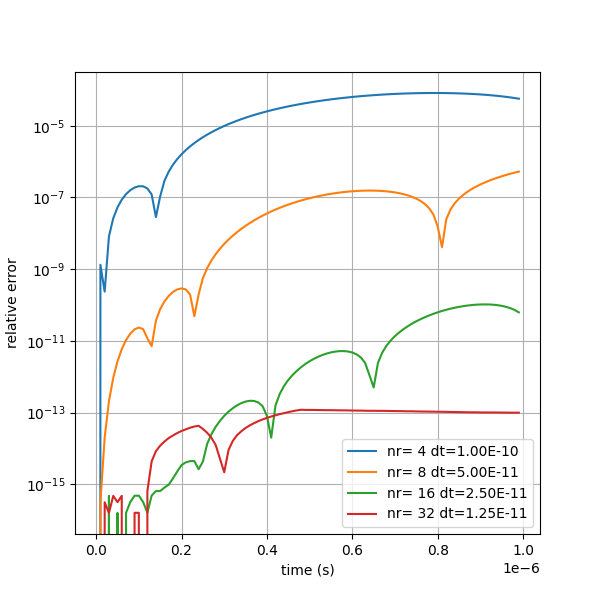
\includegraphics[width=0.32\textwidth]{fig/dat_1ev_cs_m1_temp_error.png}
	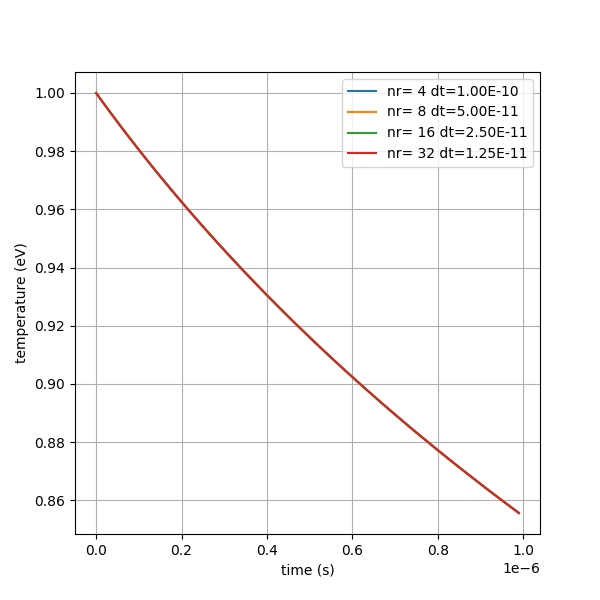
\includegraphics[width=0.32\textwidth]{fig/dat_1ev_cs_m1_temp.png}
	\caption{Mode 1}
\end{figure}
\begin{figure}[!htbp]
	\centering
	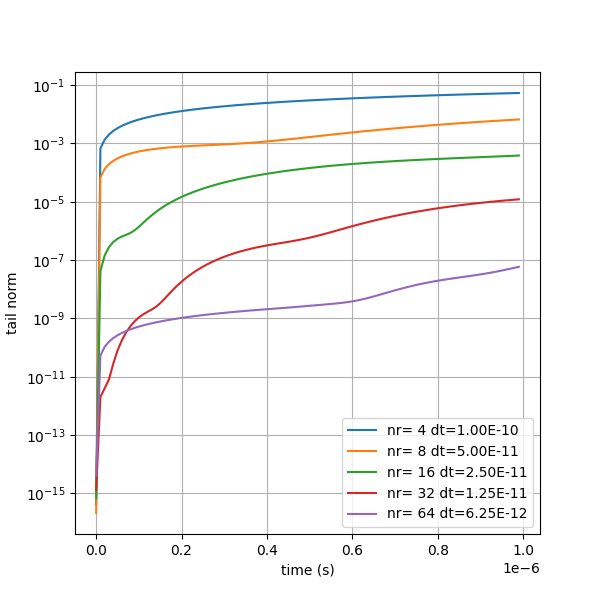
\includegraphics[width=0.32\textwidth]{fig/dat_1ev_cs_m2_tail.png}
	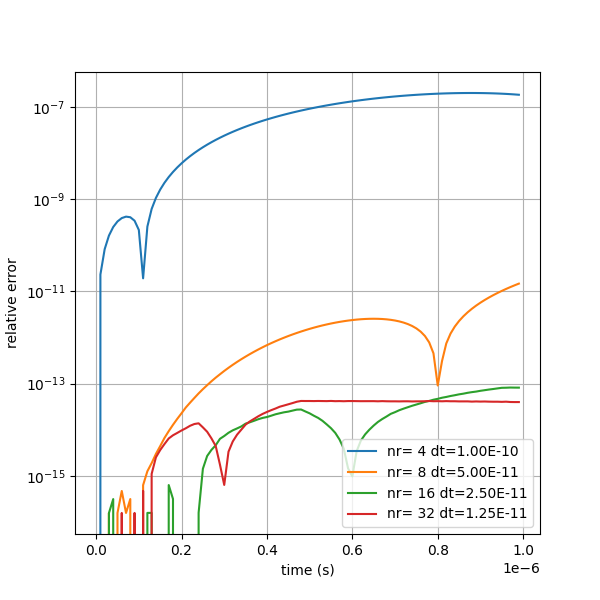
\includegraphics[width=0.32\textwidth]{fig/dat_1ev_cs_m2_temp_error.png}
	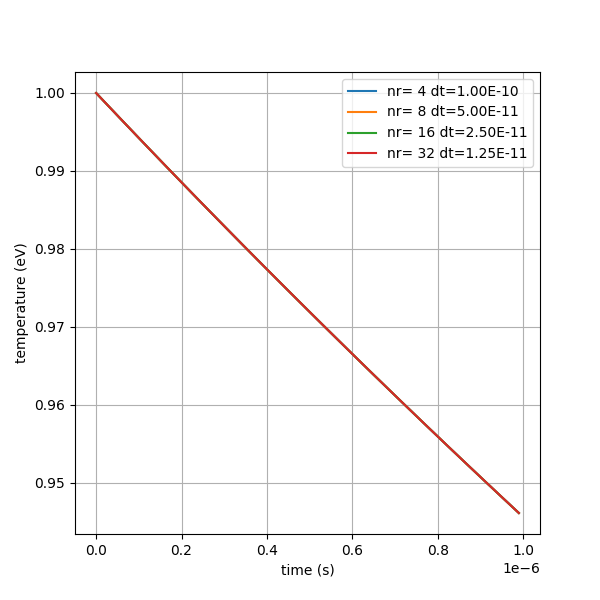
\includegraphics[width=0.32\textwidth]{fig/dat_1ev_cs_m2_temp.png}
	\caption{Mode 2}
\end{figure}
\begin{figure}[!htbp]
	\centering
	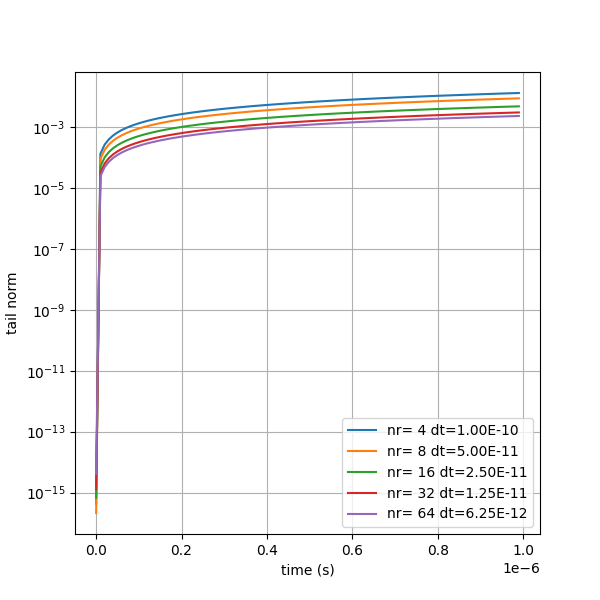
\includegraphics[width=0.32\textwidth]{fig/dat_1ev_cs_m3_tail.png}
	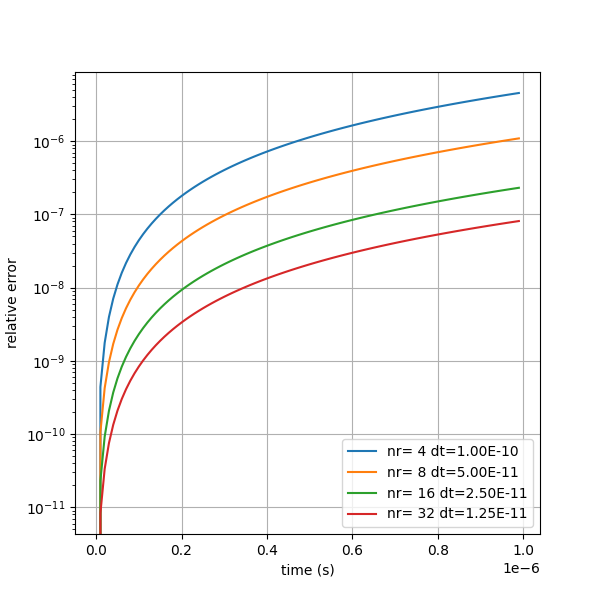
\includegraphics[width=0.32\textwidth]{fig/dat_1ev_cs_m3_temp_error.png}
	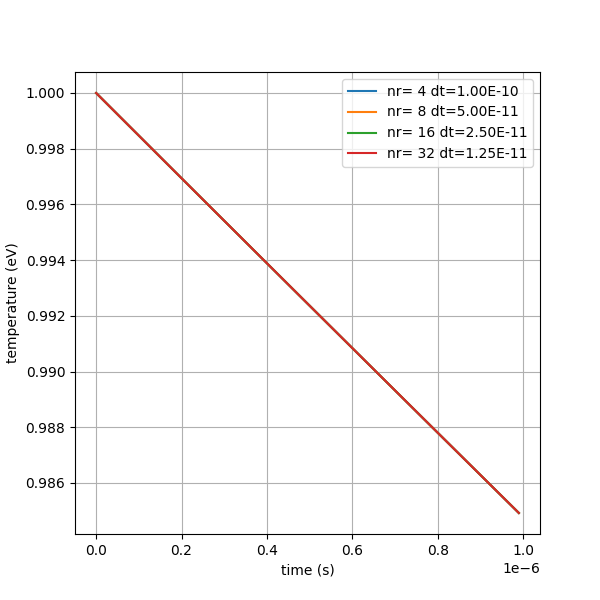
\includegraphics[width=0.32\textwidth]{fig/dat_1ev_cs_m3_temp.png}
	\caption{Mode 3}
\end{figure}
\begin{figure}[!htbp]
	\centering
	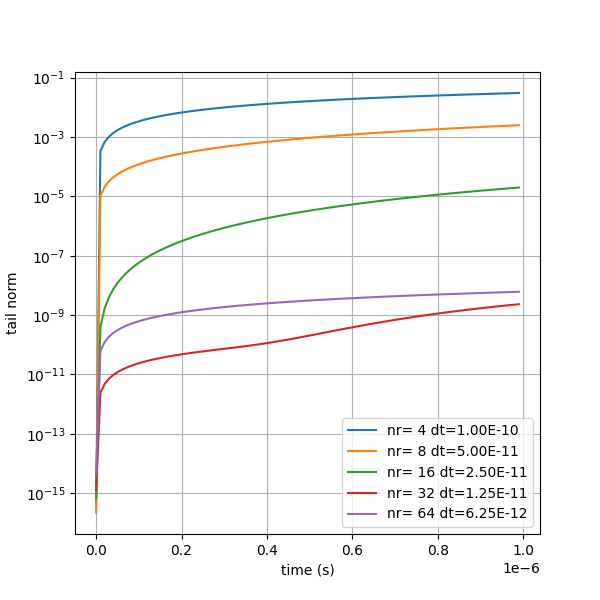
\includegraphics[width=0.32\textwidth]{fig/dat_1ev_cs_m4_tail.png}
	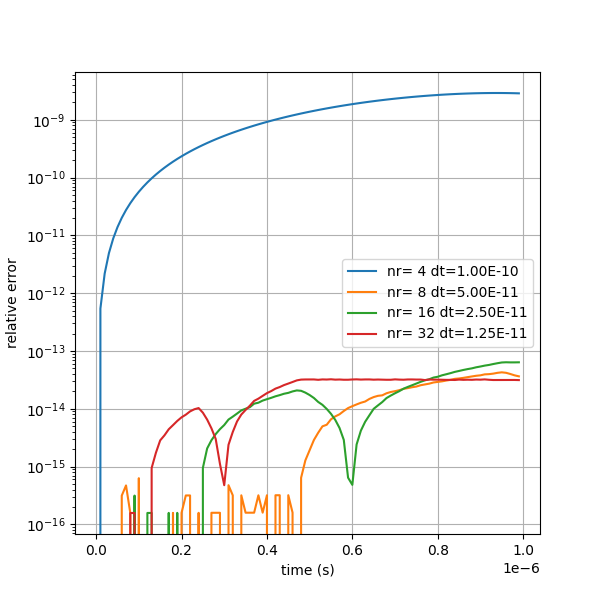
\includegraphics[width=0.32\textwidth]{fig/dat_1ev_cs_m4_temp_error.png}
	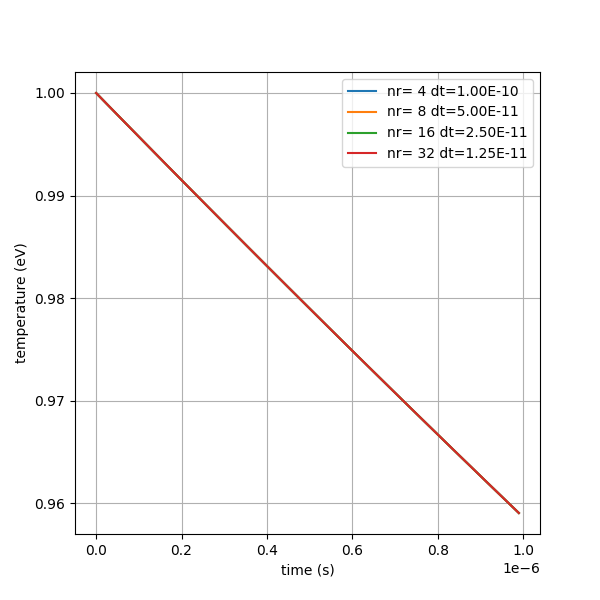
\includegraphics[width=0.32\textwidth]{fig/dat_1ev_cs_m4_temp.png}
	\caption{Mode 4}
\end{figure}
\begin{figure}[!htbp]
	\centering
	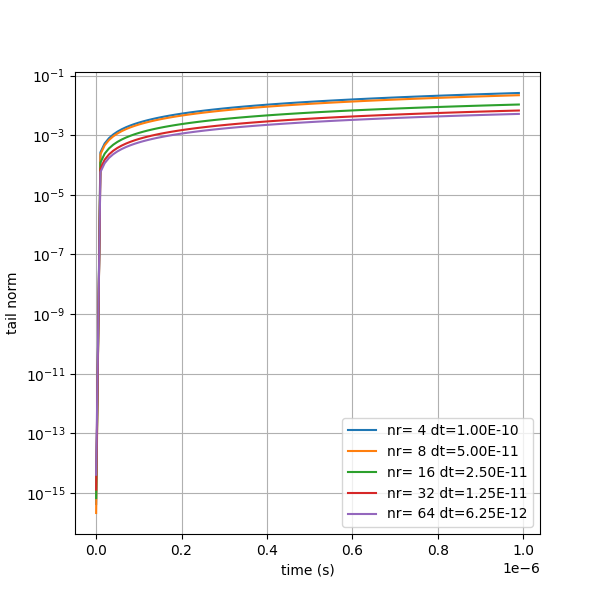
\includegraphics[width=0.32\textwidth]{fig/dat_1ev_cs_m5_tail.png}
	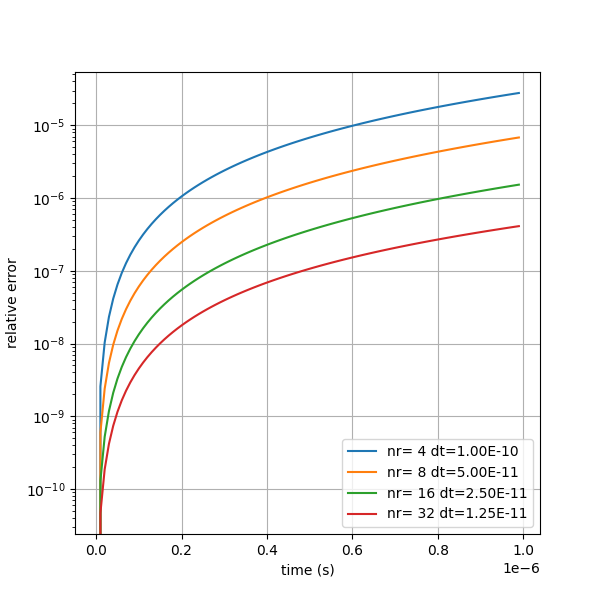
\includegraphics[width=0.32\textwidth]{fig/dat_1ev_cs_m5_temp_error.png}
	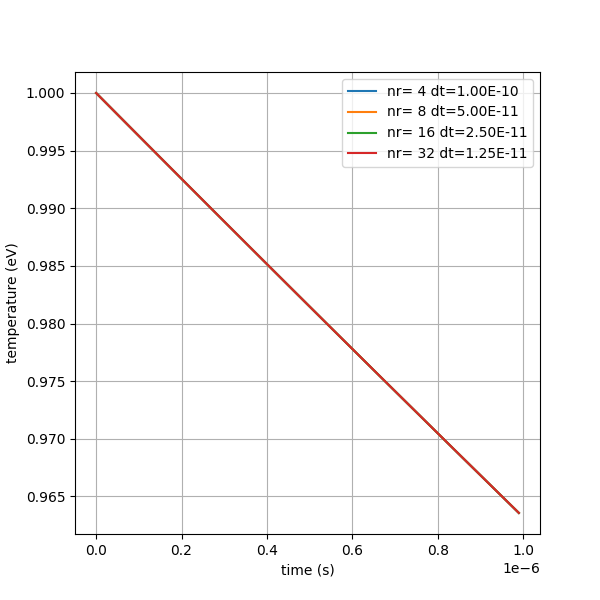
\includegraphics[width=0.32\textwidth]{fig/dat_1ev_cs_m5_temp.png}
	\caption{Mode 5}
\end{figure}
\begin{figure}[!htbp]
	\centering
	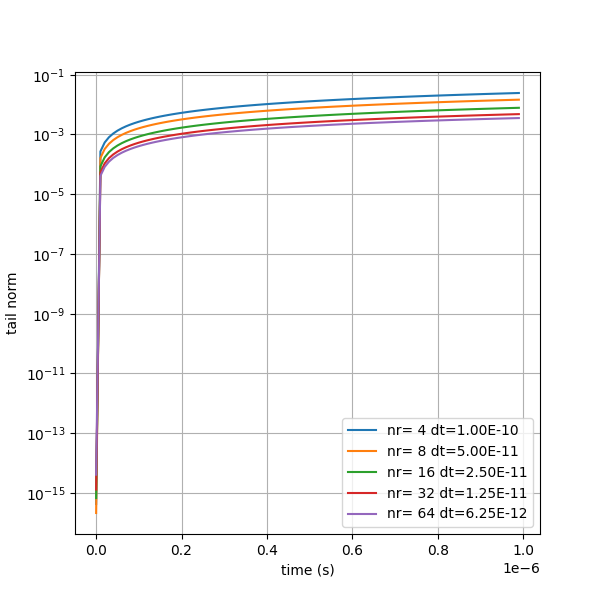
\includegraphics[width=0.32\textwidth]{fig/dat_1ev_cs_m6_tail.png}
	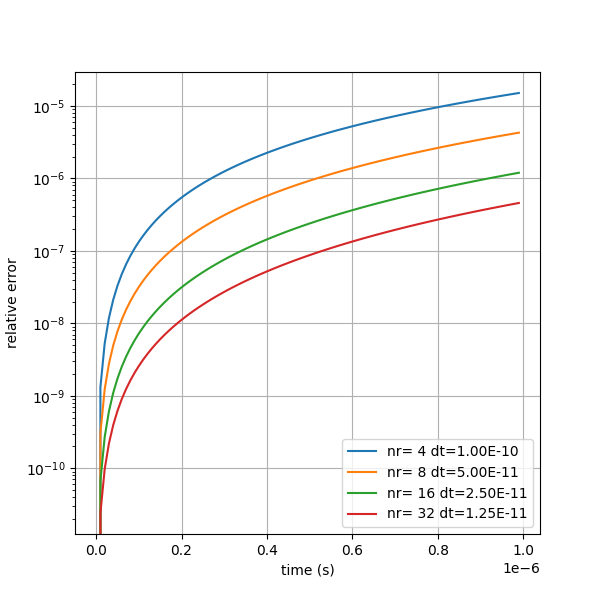
\includegraphics[width=0.32\textwidth]{fig/dat_1ev_cs_m6_temp_error.png}
	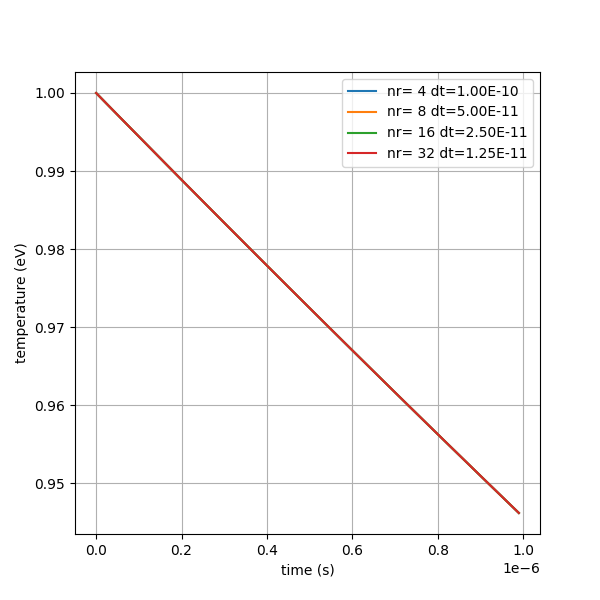
\includegraphics[width=0.32\textwidth]{fig/dat_1ev_cs_m6_temp.png}
	\caption{Mode 6}
\end{figure}
\begin{figure}[!htbp]
	\centering
	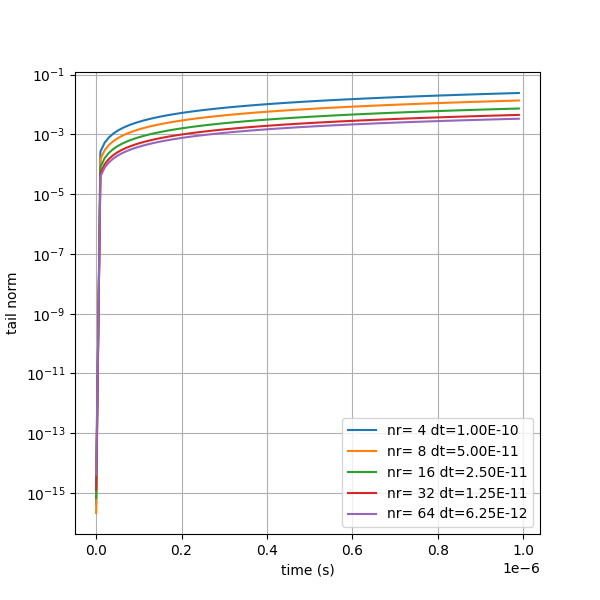
\includegraphics[width=0.32\textwidth]{fig/dat_1ev_cs_m7_tail.png}
	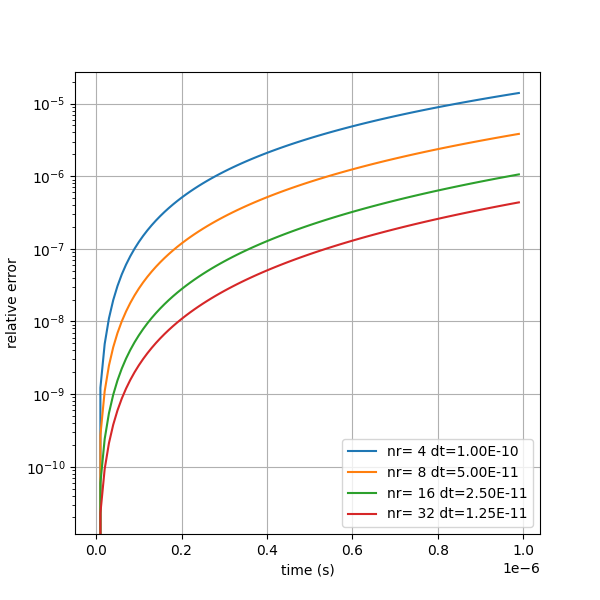
\includegraphics[width=0.32\textwidth]{fig/dat_1ev_cs_m7_temp_error.png}
	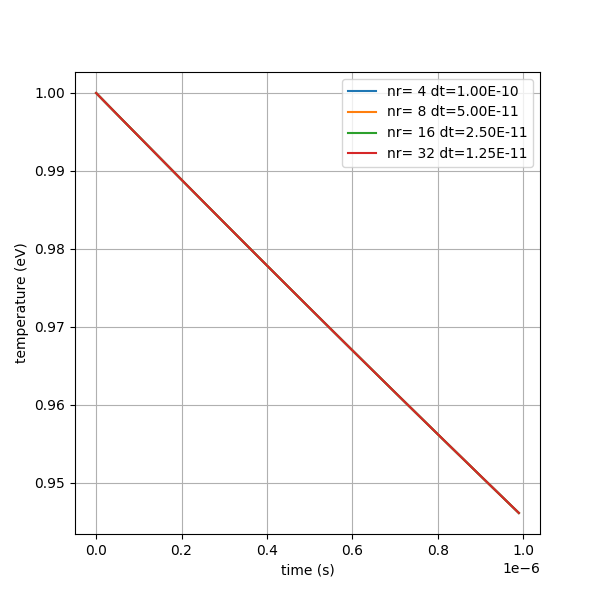
\includegraphics[width=0.32\textwidth]{fig/dat_1ev_cs_m7_temp.png}
	\caption{Mode 7}
\end{figure}

\section{Computation of the collision operator}
As described in~\S\ref{subsec:binary_reactions} we can write the binary collision operator as below.  
\begin{align*}
\myint_{R^3} C \phi\of{\vect{v}_e} \diff{\vect{v}_e} 
&=
\myint_{R^3} \myint_{R^3} \myint_{S^2} 
B\of{\vect{v}_e, \vect{v}_0, \vect{\omega}} 
f_e\of{\vect{v}_e} f_0\of{\vect{v}_0} 
\left(
\phi\of{\vect{v}_e^\text{post}\of{\vect{v}_e, \vect{v}_0, \vect{\omega}}} 
- \phi\of{\vect{v}_e} 
\right)
\diff{\vect{v}_0} \diff{\vect{v}_e} \diff{\vect{\omega}}
\end{align*}
Assuming the $f(\vect{v}_0)= n_0\delta(\vect{v}_0)$, we can simplify the above as, 
\begin{align*}
\myint_{R^3} C \phi\of{\vect{v}_e} \diff{\vect{v}_e} 
&=
n_0 \myint_{R^3} \myint_{S^2} 
B\of{\vect{v}_e, 0, \vect{\omega}} 
f_e\of{\vect{v}_e}
\left(
\phi\of{\vect{v}_e^\text{post}\of{\vect{v}_e, 0, \vect{\omega}}} 
- \phi\of{\vect{v}_e} 
\right)
\diff{\vect{v}_e} \diff{\vect{\omega}}
\end{align*}

We can try to use a fixed radial basis for each lm mode, by extracting out the $(\cdot)^{l}$ factor as follows. 
\textbf{Note} : The below basis produce ill-conditioned mass matrix. 
\begin{align*}
M(v) & = \frac{n_e}{(\sqrt{\pi}v_{th})^3} \exp{\left(-\left(\frac{v}{v_{th}}\right)^2 \right)} \\
\Phi_{klm} (\vect{v}) &= \left(\frac{v_r}{v_{th}}\right)^l \exp\left(-\left(\frac{v_r}{v_{th}}\right) ^ 2\right)  P_k\of{\frac{v_r}{v_{th}}} Y_{lm}(v_\theta,v_\phi) \\
\Psi_{pqs} (\vect{v}) &= \left(\frac{v_r}{v_{th}}\right)^q P_p\of{\frac{v_r}{v_{th}}} Y_{qs}(v_\theta,v_\phi)
\end{align*}

We can write the basis expansion for $f(\vect{v})$ as,  
\begin{align*}
f(\vect{v})  = \sum_{klm} \hat{f}_{klm} \Phi_{klm} (\vect{v})
\end{align*}
Then the discretized collision operator becomes, 
\begin{align*}
{L}_{k,l,m}^{p,q,s} &=n_0 \myint_{0}^{+\infty} \myint_{S^2} \myint_{S^2} v_r^2 \norm{\vect{v}} \sigma(\vect{v},\omega) \Phi_{klm}(\vect{v})   (\Psi_{pqs}(\vect{v}_e^{post}(\vect{v},\omega)) - \Psi_{pqs}(\vect{v})) \diff{\omega} \diff{\omega_v} \diff{v_r} \\
{L}_{k,l,m}^{p,q,s} &=n_0 (v_{th})^3 \myint_{0}^{+\infty} \myint_{S^2} \myint_{S^2} \left(\frac{v_r}{v_{th}}\right)^{(2+l)} \norm{\vect{v}} \sigma(\vect{v},\omega) \exp\left(-\left(\frac{v_r}{v_{th}}\right) ^ 2\right) \\
&P_k\of{\frac{v_r}{v_{th}}} Y_{lm}(v_\theta,v_\phi)  (\Psi_{pqs}(\vect{v}_e^{post}(\vect{v},\omega)) - \Psi_{pqs}(\vect{v})) \diff{\omega} \diff{\omega_v} \frac{\diff{v_r}}{v_{th}} \\
{M}_{k,l,m}^{p,q,s} &= \myint_{0}^{+\infty} \myint_{S^2} \myint_{S^2}  v_r^2 \Psi_{pqs}(\vect{v}) \Phi_{klm}(\vect{v}) \diff{\omega} \diff{\omega_v} \diff{v_r}\\
{M}_{k,l,m}^{p,q,s} &= (v_{th})^3 \myint_{0}^{+\infty} \myint_{S^2} \myint_{S^2} 
\left(\frac{v_r}{v_{th}}\right)^{(2+l+q)} P_p\of{\frac{v_r}{v_{th}}} Y_{qs}(v_\theta,v_\phi) \exp\left(-\left(\frac{v_r}{v_{th}}\right) ^ 2\right)  \\& P_k\of{\frac{v_r}{v_{th}}} Y_{lm}(v_\theta,v_\phi) \diff{\omega} \diff{\omega_v} \frac{\diff{v_r}}{v_{th}}
\end{align*}

Using orthogonalized radial basis for each lm mode we can discretize the collision operator as follows. 
\begin{align*}
M(v) & = \frac{n_e}{(\sqrt{\pi}v_{th})^3} \exp{\left(-\left(\frac{v}{v_{th}}\right)^2 \right)} \\
\Phi_{klm} (\vect{v}) &= \exp\left(-\left(\frac{v_r}{v_{th}}\right) ^ 2\right)  P_{kl}\of{\frac{v_r}{v_{th}}} Y_{lm}(v_\theta,v_\phi) \\
\Psi_{pqs} (\vect{v}) &= P_{pq}\of{\frac{v_r}{v_{th}}} Y_{qs}(v_\theta,v_\phi)
\end{align*} where, 
\begin{align*}
P_{pq}\of{x}  &= x^q \mathcal{P}^{2q+2}_p(x)  \\
\myint_{0}^{+\infty} P_{pq}\of{x} P_{pl} \exp(-x^2) x^2 dx &= \delta_{ql}
\end{align*} with $\mathcal{P}^{2q+2}_p$ denotes the derived Maxwell polynomials. 


\begin{align*}
{L}_{k,l,m}^{p,q,s} &=n_0 (v_{th})^3 \myint_{0}^{+\infty} \myint_{S^2} \myint_{S^2} \left(\frac{v_r}{v_{th}}\right)^{2} \norm{\vect{v}} \sigma(\vect{v},\omega) \exp\left(-\left(\frac{v_r}{v_{th}}\right) ^ 2\right) \\
&P_{kl}\of{\frac{v_r}{v_{th}}} Y_{lm}(v_\theta,v_\phi)  (\Psi_{pqs}(\vect{v}_e^{post}(\vect{v},\omega)) - \Psi_{pqs}(\vect{v})) \diff{\omega} \diff{\omega_v} \frac{\diff{v_r}}{v_{th}} \\
{M}_{k,l,m}^{p,q,s} &= (v_{th})^3 \myint_{0}^{+\infty} \myint_{S^2} \myint_{S^2} 
\left(\frac{v_r}{v_{th}}\right)^{2} P_{pq}\of{\frac{v_r}{v_{th}}} Y_{qs}(v_\theta,v_\phi) \exp\left(-\left(\frac{v_r}{v_{th}}\right) ^ 2\right)  \\& P_{kl}\of{\frac{v_r}{v_{th}}} Y_{lm}(v_\theta,v_\phi) \diff{\omega} \diff{\omega_v} \frac{\diff{v_r}}{v_{th}} \\
{M}_{k,l,m}^{p,q,s} &= \delta^p_q \delta^q_l \delta^m_s
\end{align*}

For given distribution function of the form, $f(\vect{v}) = \exp\of{-\left(\frac{v_r}{v_{th}}\right)^2}h(\vect{v})$ we can compute the expansion coefficients $\hat{f}_{klm}$ as, 
\begin{align*}
\hat{f}_{klm} = \myint_{R^3} \Psi_{klm}(\vect{v}) f(\vect{v}) \diff{\vect{v}}
\end{align*}

The $n^{th}$ moment of the distribution function can be computed,
\begin{align*}
m_n&=\myint_{R^3} \norm{v}^n f(\vect{v}) \diff{\vect{v}}\\
m_n&=(v_{th})^{3+n}\myint_{0}^{+\infty} \myint_{S^2} \of{\frac{v_r}{v_{th}}}^{2+n} \sum_{klm} \hat{f}_{klm} \Phi_{klm}(\vect{v}) \diff{\omega}\frac{\diff{v_r}}{v_{th}}
\end{align*}

The electron temperature is defined as, 
\begin{align*}
T_e & = \frac{1}{3k_B} m_e \frac{m_2}{m_0}
\end{align*}
The electron energy distribution function (EEDF) can be computed with, 
\begin{align*}
E_f(\epsilon) &= \myint_{S^2} f\of{\left(\sqrt{\frac{2\epsilon}{m_e}},\omega\right)} \diff{\omega} \\
E_f(\epsilon) &= \myint_{S^2} \sum_{klm} \exp(-\frac{2\epsilon}{m_e}) \hat{f}_{klm} \Phi_{klm}\of{\left(\sqrt{\frac{2\epsilon}{m_e}},\omega\right)} \diff{\omega}
\end{align*}

%\subsection{Collision operator using B-splines}
%\begin{align*}
%M(v) & = \frac{n_e}{(\sqrt{\pi}v_{th})^3} \exp{\left(-\left(\frac{v}{v_{th}}\right)^2 \right)} \\
%\Phi_{klm} (\vect{v}) &= \left(\frac{v_r}{v_{th}}\right)^l P_k\of{\frac{v_r}{v_{th}}} Y_{lm}(v_\theta,v_\phi) \\
%\Psi_{pqs} (\vect{v}) &= \left(\frac{v_r}{v_{th}}\right)^q P_p\of{\frac{v_r}{v_{th}}} Y_{qs}(v_\theta,v_\phi)
%\end{align*}where $P_k,P_p$ denotes the B-splines polynomials.  

\textbf{Spectrum of the collision operator} : Let $C : V \rightarrow V$ denotes the infinity dimension collision operator, $P_n V \rightarrow V_n$ be the projection operator for finite dimensional subspace $V_n \subset V$. For orthogonal radial basis choice, $P_n$ is an orthogonal projection, while for B-splines it is not orthogonal.
\begin{align*}
C_{n\times n} &= P_n C P_n^T \\
\norm{C_{n\times n}} = \norm{P_n C P_n^T} &\leq \norm{P_n^2}\norm{C} \\
\norm{P_n} &=\sqrt{n} \\
\frac{\norm{C_{n\times n}}}{n} &\leq \norm{C}
\end{align*}

\subsection{Tensorized computation of ${L}_{k,l,m}^{p,q,s}$}

%\begin{align*}
%    {L}_{k,l,m}^{p,q,s} &= {L^{+}}_{k,l,m}^{p,q,s} - {L^{-}}_{k,l,m}^{p,q,s}
%\end{align*} where, 
%\begin{align*}
%    {L^{+}}_{k,l,m}^{p,q,s} = n_0 \int_{v_r} 
%                               \int_{S^2(v_\theta,v_\phi)}
%                               \int_{S^2(\chi,\gamma)} & 
%                               v^2 M(v^\prime) P^p \of{\frac{v}{\vth}} Y^{qs}\of{v_\theta, v_\phi} \times \\ & P_k\of{\frac{v^\prime}{\vth}} Y_{lm}\of{v_\theta^\prime, v_\phi^\prime} |v|\sigma(|v|,\chi) d\omega d\omega_v dv \\
%    {L^{-}}_{k,l,m}^{p,q,s} = n_0 \int_{v_r} 
%                              \int_{S^2(v_\theta,v_\phi)}
%                              \int_{S^2(\chi,\gamma)} & 
%                              v^2 M(v) P^p \of{\frac{v}{\vth}} Y^{qs}\of{v_\theta, v_\phi} \times \\ & P_k\of{\frac{v}{\vth}} Y_{lm}\of{v_\theta, v_\phi} |v|\sigma(|v|,\chi) d\omega d\omega_v dv
%\end{align*}

The list of tensors that can be precomputed
\begin{itemize}
	\item $V_r$ - quadrature points on the radial direction (incident velocities)
	\item $W_r$ - quadrature weights on the radial direction
	\item $V_\theta$ - quadrature points on the polar direction 
	\item $W_\theta$ - quadrature weights for theta
	\item $V_\phi$ - quadrature points on the azimuthal direction 
	\item $S_\chi$ - quadrature points on the scattering angle
	\item $S_\gamma$ - quadrature points on the azimuthal angle (for scattering direction)
	\item $W_\chi$ - quadrature weights
	\item $\sigma_{r\chi}$ - differential cross section tensor (rank 2)
	\item $Y_{lm}^{\theta\phi}$ - $lm$-mode spherical harmonic function evaluated at $(V_\theta, V_\phi)$. The sparse version (i.e., for given $l$ mode not selecting all the $m$ modes) , but generally can be considered as rank 4 tensor. 
	\item $M_r$ - Maxwellian times $v_r$ evaluated at $V_r$
	\item $P_{kr}$     - $k^{th}$ Maxwell polynomial evaluated at the $V_r$ $r^{th}$ location.
\end{itemize}
Notation : Same index up-down denotes contraction, $\otimes$ for kronecker product, same level index, same index (i.e., up-up, down down) denotes the element-wise multiplication. 
The total cross section $\sigma_r$, can be written as, 
\begin{align}
\sigma_r &= \frac{\pi}{|S\chi|} \sigma_{r,\chi} W^\chi
\end{align}

The weighted spherical harmonic tensor, 
\begin{align}
\tilde{Y}^{qsr}_{\theta\phi} = \mleft({Y}^{qs}_{\theta\phi} W_\theta \frac{\pi}{|V\chi|} \mright) 
\end{align}

Then we can write, 
\begin{align}
{L^{-}}_{k,l,m}^{p,q,s} &= ((P^p_r W_r \sigma_r) (P^r_k M^r) ) \otimes Y_{lm}^{\theta\phi} \tilde{Y}^{qs}_{\theta\phi} \\
{L^{-}}_{k,l,m}^{p,q,s} &= ((P^p_r W_r \sigma_r) (P^r_k M^r) ) \otimes \delta^{qs}\delta_{lm} %Y_{lm}^{\theta\phi} \tilde{Y}^{qs}_{\theta\phi} 
\end{align}


More additional tensors that we need to compute the $L^{+}$ component. 

\begin{itemize}
	\item $S^{r\theta\phi\chi\gamma}_{r^\prime\theta^\prime \phi^\prime}$ : Scattering velocity tensor, for each $v=(r,\theta,\phi)$ and scattering solid angle $(\chi,\gamma)$ computes $(r^\prime,\theta^\prime,\phi^\prime)$ scattered or newly created particle velocity (i.e., in G2 ejected electron). This is a rank 8 tensor where it might be too expensive to compute. For cases $G0$, $G1$ we can compute $S^{r\theta\phi\chi\gamma}_{r^\prime\theta^\prime \phi^\prime} = {S^r}_{r^\prime} \otimes S^{\theta\phi\chi\gamma}_{\theta^\prime \phi^\prime}$ since radial component only depends on energy, while for reactions like $G2$ it's depends on both energy and direction (i.e., for momentum conservation).
	\item $P^{r\theta\phi\chi\gamma}_{k}$ - radial polynomial evaluated at differed velocity for given incident particle ($r,\theta,\phi,\chi,\gamma$)
	\item $M^{r\theta\phi\chi\gamma}$ - Maxwellian times $v_r$ evaluated for the differed particle for a given incident particle ($r,\theta,\phi,\chi,\gamma$)
	\item $Y^{r\theta\phi\chi\gamma}_{lm}$ - $lm$ spherical harmonic mode evaluated differed particle direction for a given incident particle ($r,\theta,\phi,\chi,\gamma$)
	\item $\sigma^{r\theta\phi\chi\gamma}$ - differential cross section broadcasted on scattering cross section angles. 
	\item $B^{r\theta\phi}_{pqs}$ - $pqs$ basis evaluated at the incident grid.              
\end{itemize}

For the general case, of the differed particle, (i.e., differed particle all velocity components are functions of $r,\theta,\phi,\chi,\gamma$) we can write the following. Note, $A$ is obtained for contraction on the $\gamma$ azimuthal of angle of the scattered particle, $B$ is obtained with contraction on the polar angle of the scattering direction, $C$ is obtained contraction on $(\theta,\phi)$ for the velocity space angular directions, and finally $L^{+}$ obtained using radical direction contraction. 

\begin{align}
A^{r\theta\phi}_{klm}   &=  ( P^{r\theta\phi\chi\gamma}_{k} M^{r\theta\phi\chi\gamma} Y^{r\theta\phi\chi\gamma}_{lm}) W{\gamma} W_{\chi} \\
{L^{+}}_{k,l,m}^{p,q,s} &=  B^{r\theta\phi}_{pqs} A^{r\theta\phi}_{klm} W_\phi W_\theta W_r
% B^{r\theta\phi}_{klm}      & = \frac{\pi}{|S_\gamma|} \sigma^{r\chi} (W_\chi A^{r\theta\phi}_{\chi klm}) \\
% C^{rqs}_{klm}              & = \tilde{Y}^{qs}_{\theta\phi} B^{r\theta\phi}_{klm} \\
%{L^{+}}_{k,l,m}^{p,q,s}     & = {P^p}_r C^{rqs}_{klm}
\end{align}

\subsection{Distribution moments in basis expansion}
Let $f(v) = M(v_\alpha) \sum_{klm} f_{klm} \phi_{klm}(v_\alpha)$, where $v_\alpha = v/\alpha$. Then we can write the zeroth moment (number of species particles) of the distribution, 
\begin{align}
n_e & = \int_{R^3} f(v) dv \\
\end{align} which can be written as, 
\begin{align}
n_e & = q^{klm} f_{klm}  
\end{align} where, 
\begin{align}
q_{klm} & = \int_{\R^3} M(v_\alpha) \phi_{klm}(v_\alpha) dv = 0  \text{ if } klm \neq 000 \\
q_{000} & = \int_{\R^3} M(v_\alpha) \phi_{klm}(v_\alpha) dv = \frac{n}{4\pi} 
\end{align}


\subsection{Varying thermal velocity}
Let $\alpha,\beta$ be two thermal velocities, and their corresponding normalized velocity be $v_\alpha=v/\alpha,v_\beta=v/\beta$.
Let $f(v) = M(v_\alpha) h(v_\alpha)$. Let $h^{(\alpha)}$ be the basis coefficients w.r.t. the chosen basis. Let us try to expand $f(v)$ using maxwellian at different temperature say at $\beta$, let $h^{(\beta)}$ be the coefficients for the expansion.
\begin{equation}
M^{(\beta)} h^{(\beta)} = W^{(\alpha)} h^{(\alpha)}
\end{equation} where, 
\begin{align}
M^{(\beta)}_{ij} &= \int_{v} \int_{S^2} M(v_\beta) \phi_i(v_\beta) \phi_j(v_\beta) d\omega dv  = \frac{n}{4\pi} \delta_{ij} \\
W^{(\alpha)}_{ij} &= \int_{v} \int_{S^2} M(v_\alpha) \phi_i(v_\beta) \phi_j(v_\alpha) d\omega dv   \label{eq:bchnage}
\end{align}

For $W_ij^{(\alpha)}$, let i=0, then we can write (Note : $\phi_0(v_\beta)=1$)
\begin{align*}
W^{(\alpha)}_{0j} &= \int_{v} \int_{S^2} M(v_\alpha) \phi_0(v_\beta) \phi_j(v_\alpha) d\omega dv\\
W^{(\alpha)}_{0j} &= \int_{v} \int_{S^2} M(v_\alpha) \phi_j(v_\alpha) d\omega dv = \frac{n}{4\pi} \delta_{0j}
\end{align*}
Therefore, we can write $h^{(\beta)}_0=h^{(\alpha)}_0$. There zeroth coefficient always match hence we should preserve zeroth moment of the distribution under basis change.  

\subsection{Bounds on the tails for the basis change}
The thermal velocity basis change operator is given by, \eqref{eq:bchnage}, using orthogonality in the angular directions we can only operate in the radial direction. Therefore, the above simplifies to following (note that we can consider scaling of the 1d Maxwellian)
\begin{align}
W_{ij} &= \int_{\reals} M(v_\alpha) P_i(v_\beta) P_j(v_\alpha)dv \label{eq:basis_change}
\end{align}
Let $\epsilon >0$, $\alpha = \beta + \epsilon$. Then we can write the simplified $W_{ij}$ as, 
\begin{align}
W_{ij} &= \frac{n}{\sqrt{\pi}^{3}}  \int_{\reals}  \exp(-v_\alpha^2) P_i (v_\alpha (1 + \frac{\epsilon}{\beta})) P_j(v_\alpha) \frac{dv}{\alpha} \\
\end{align}